\section{Resultado final}

Los instantes más importantes de la animación final, quitando el movimiento de la cámara para más claridad, son:

\begin{figure}[H]
    \centering 
\begin{subfigure}[t]{0.48\textwidth}
    \centering
    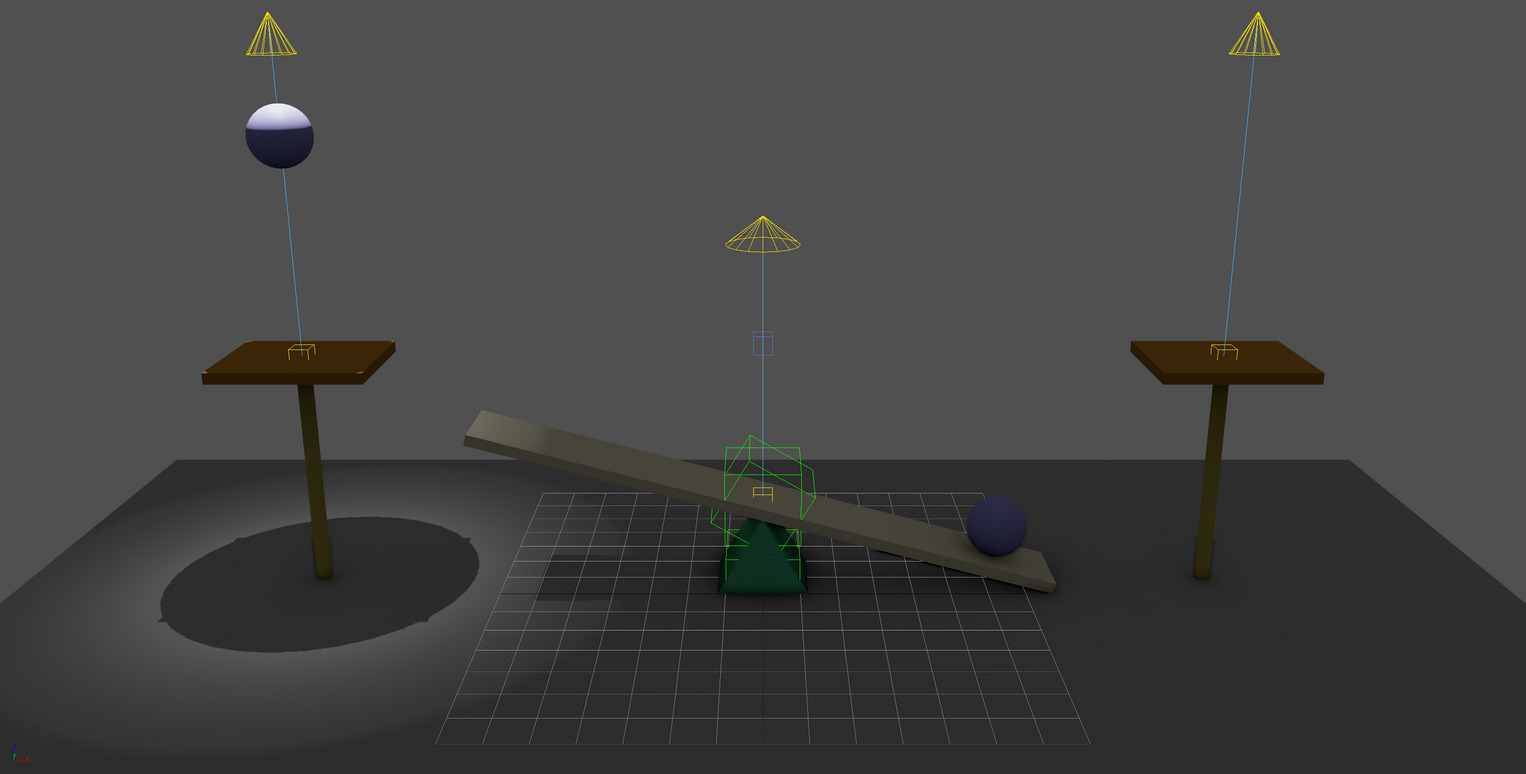
\includegraphics[width=\textwidth]{imagenes/animaciones/general/0.jpg}
    \caption{Animación de la escena en el instante 0.}
 \end{subfigure}
\hfill
 \begin{subfigure}[t]{0.48\textwidth}
    \centering
    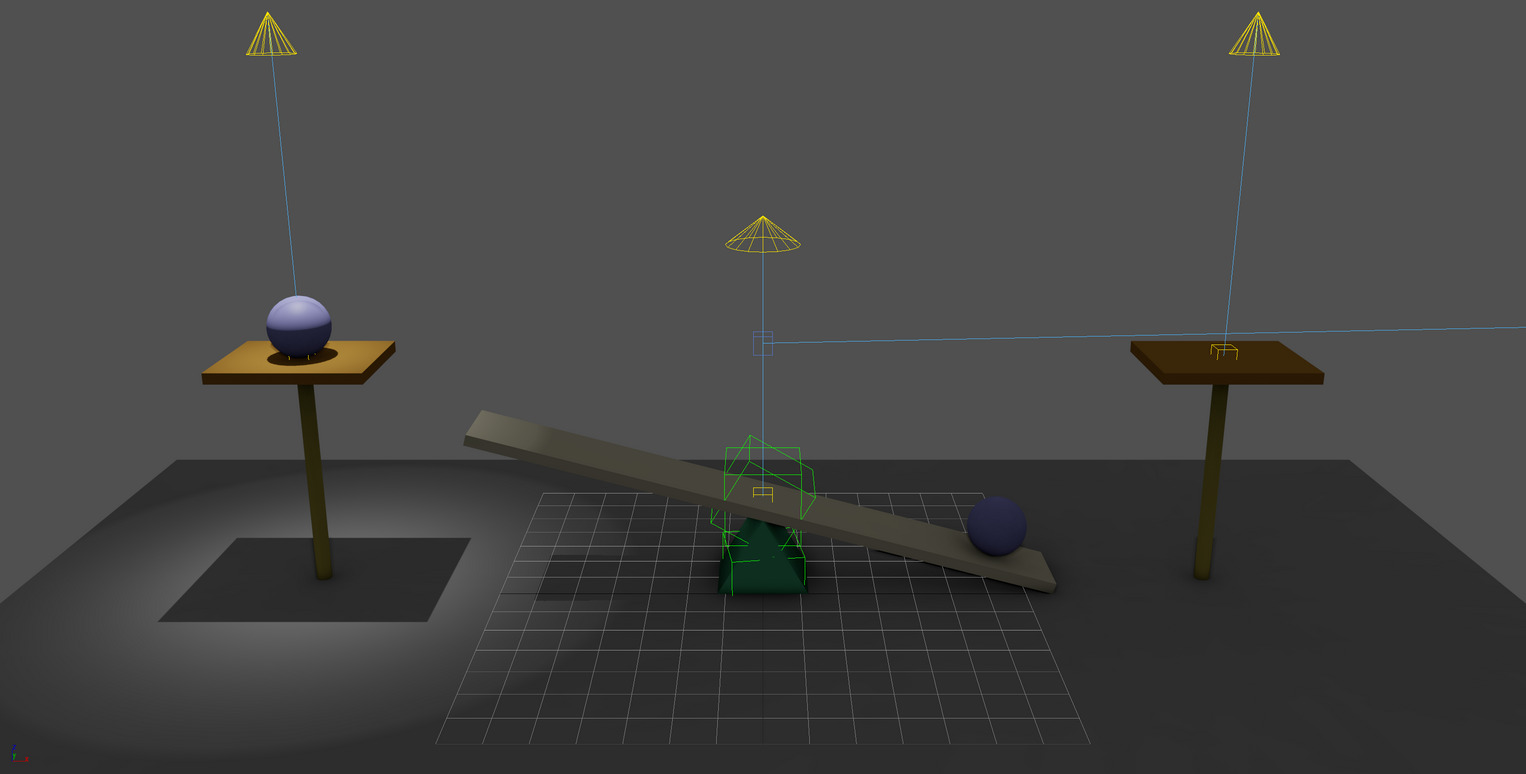
\includegraphics[width=\textwidth]{imagenes/animaciones/general/14.jpg}
    \caption{Animación de la escena en el instante 14.}
 \end{subfigure}
\hfill
 \begin{subfigure}[t]{0.48\textwidth}
    \centering
    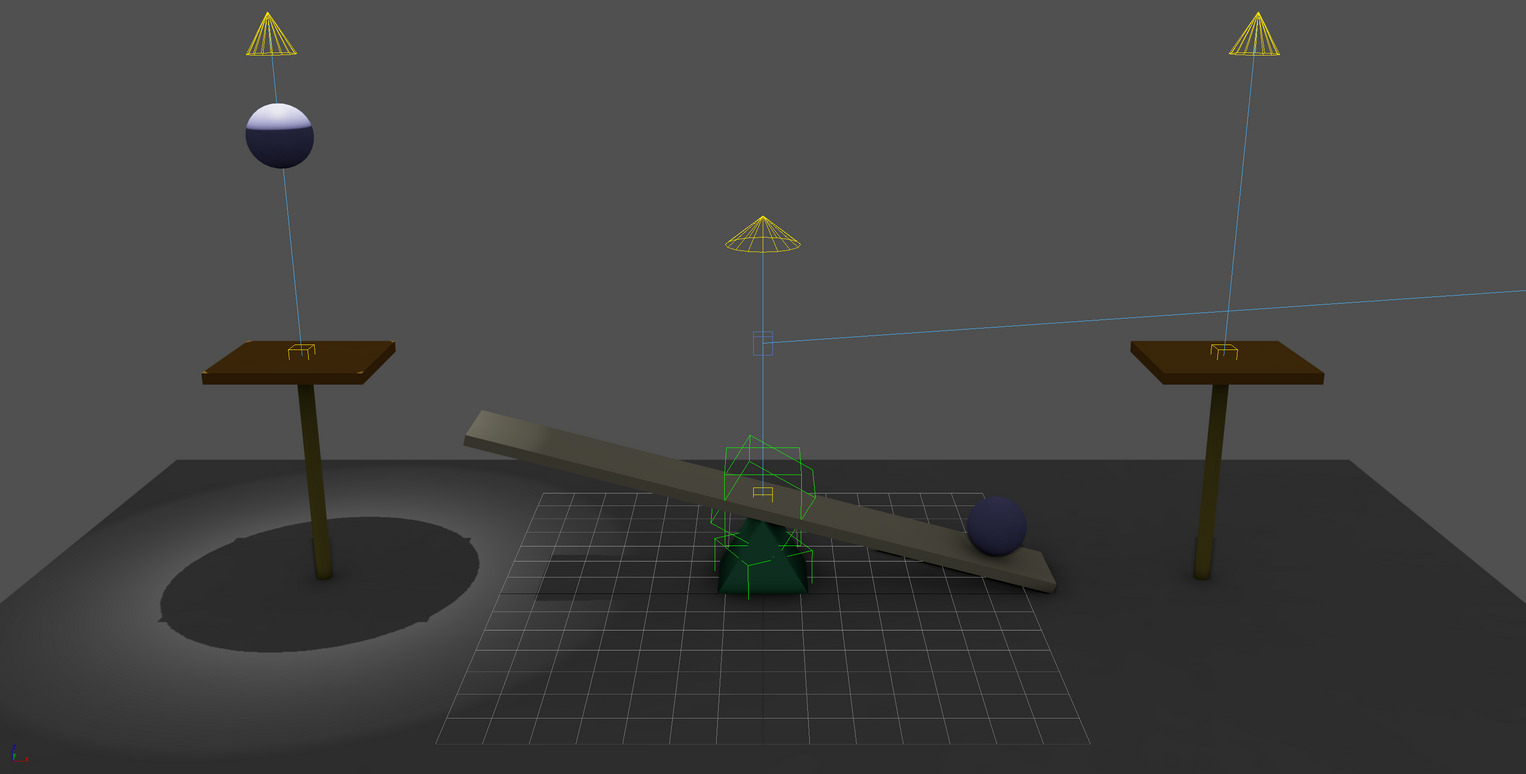
\includegraphics[width=\textwidth]{imagenes/animaciones/general/26.jpg}
    \caption{Animación de la escena en el instante 26.}
 \end{subfigure}
\hfill
 \begin{subfigure}[t]{0.48\textwidth}
    \centering
    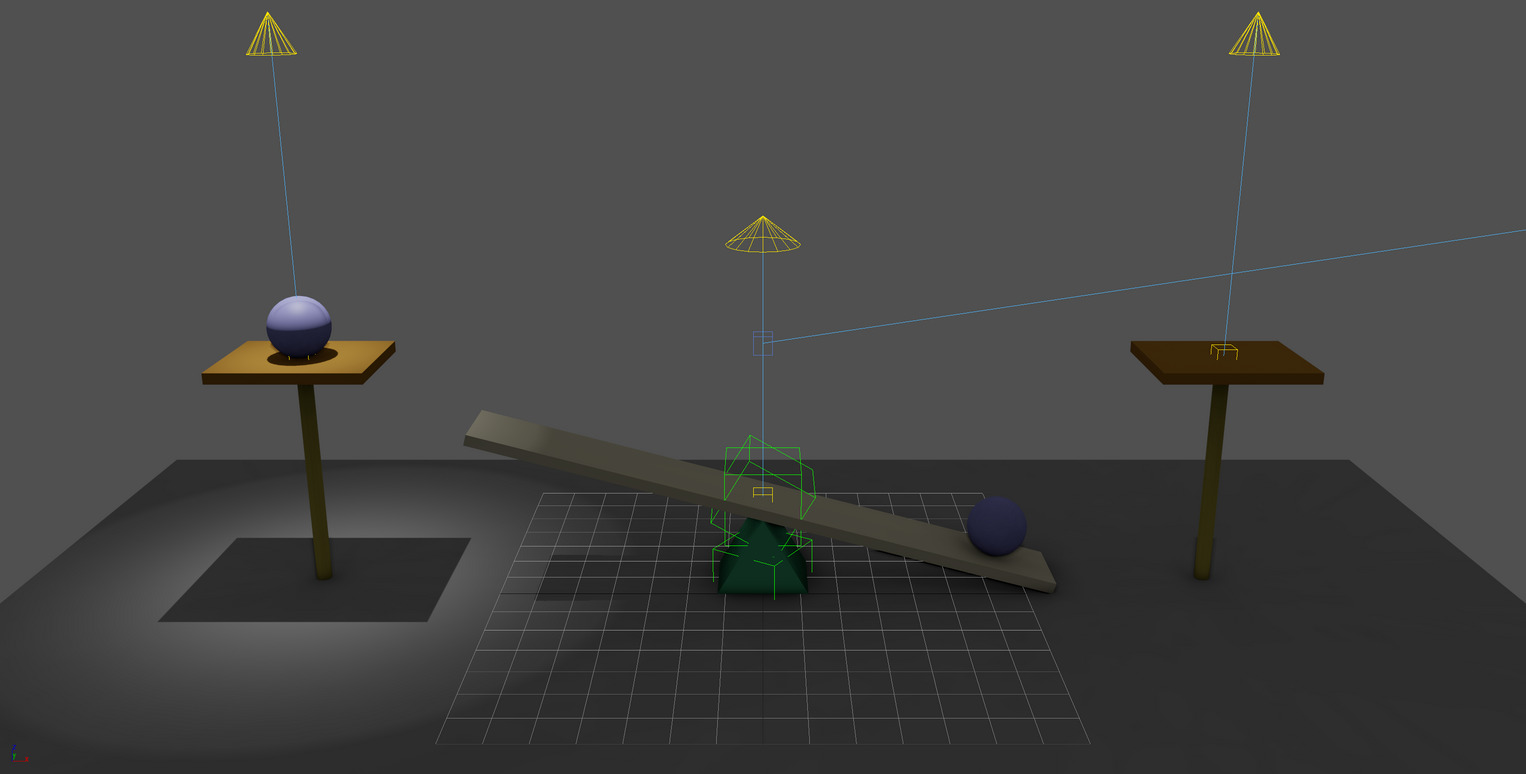
\includegraphics[width=\textwidth]{imagenes/animaciones/general/38.jpg}
    \caption{Animación de la escena en el instante 38.}
 \end{subfigure}
\hfill
 \begin{subfigure}[t]{0.48\textwidth}
    \centering
    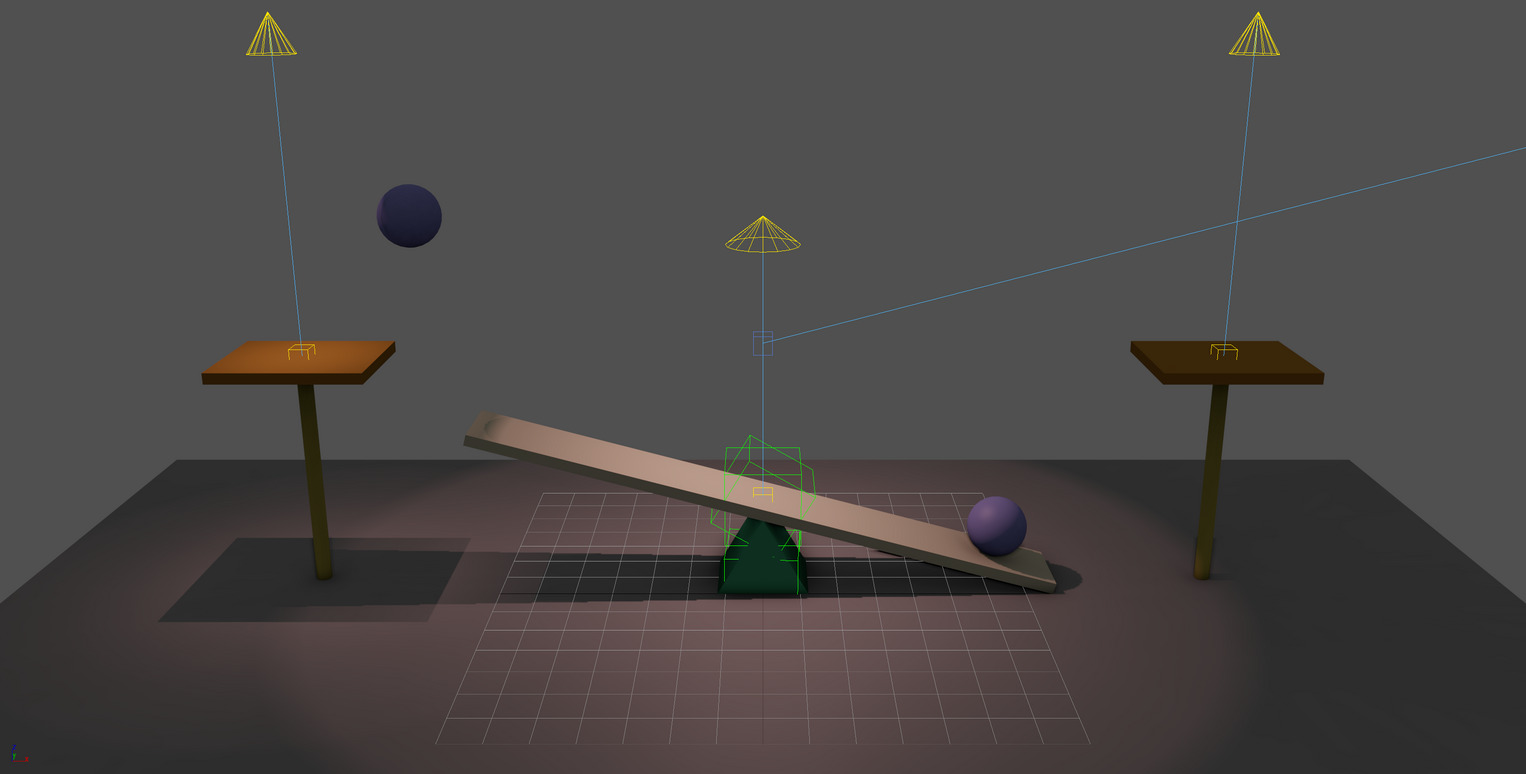
\includegraphics[width=\textwidth]{imagenes/animaciones/general/48.jpg}
    \caption{Animación de la escena en el instante 48.}
 \end{subfigure}
\hfill
 \begin{subfigure}[t]{0.48\textwidth}
    \centering
    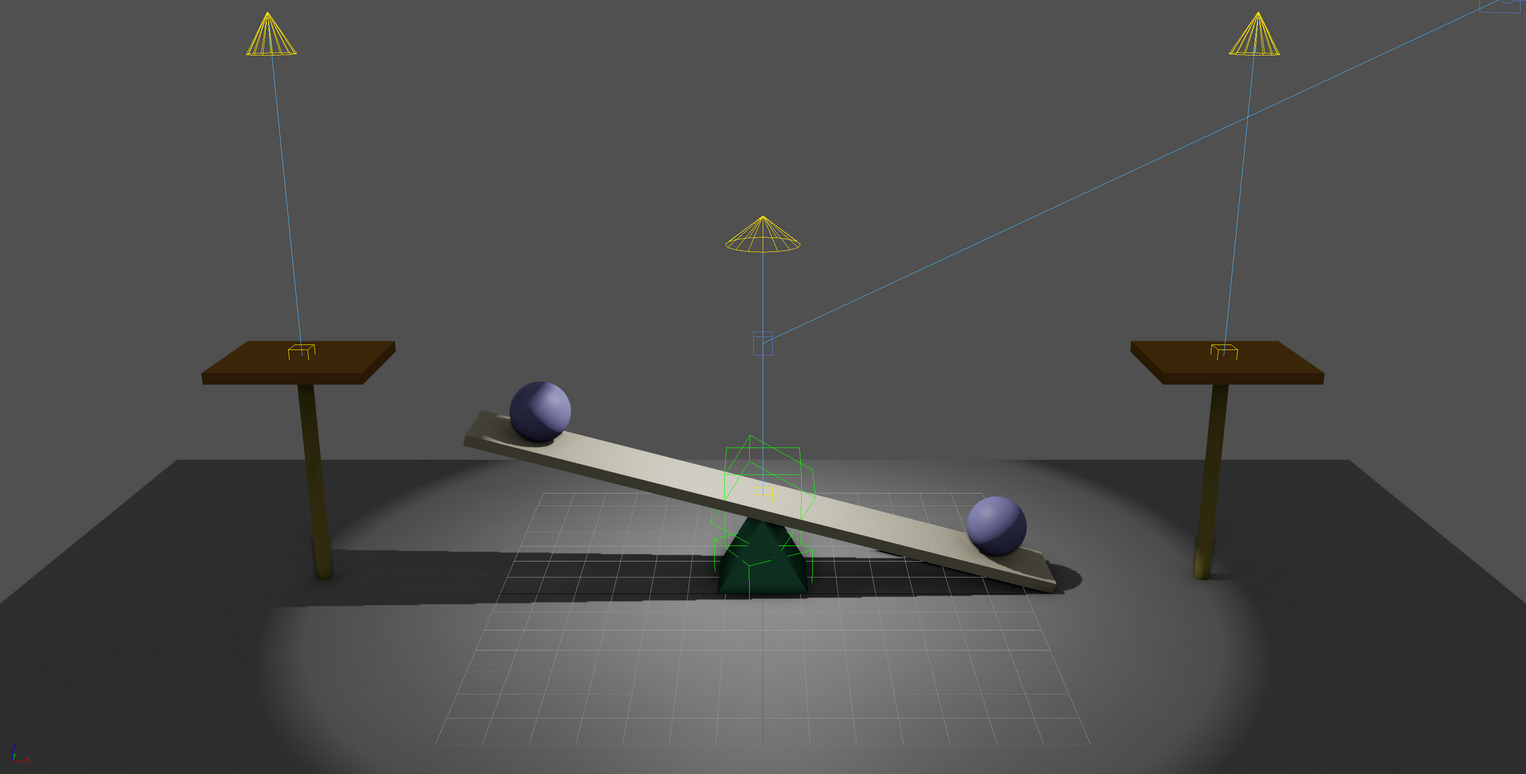
\includegraphics[width=\textwidth]{imagenes/animaciones/general/58.jpg}
    \caption{Animación de la escena en el instante 58.}
 \end{subfigure}
\hfill
 \begin{subfigure}[t]{0.48\textwidth}
    \centering
    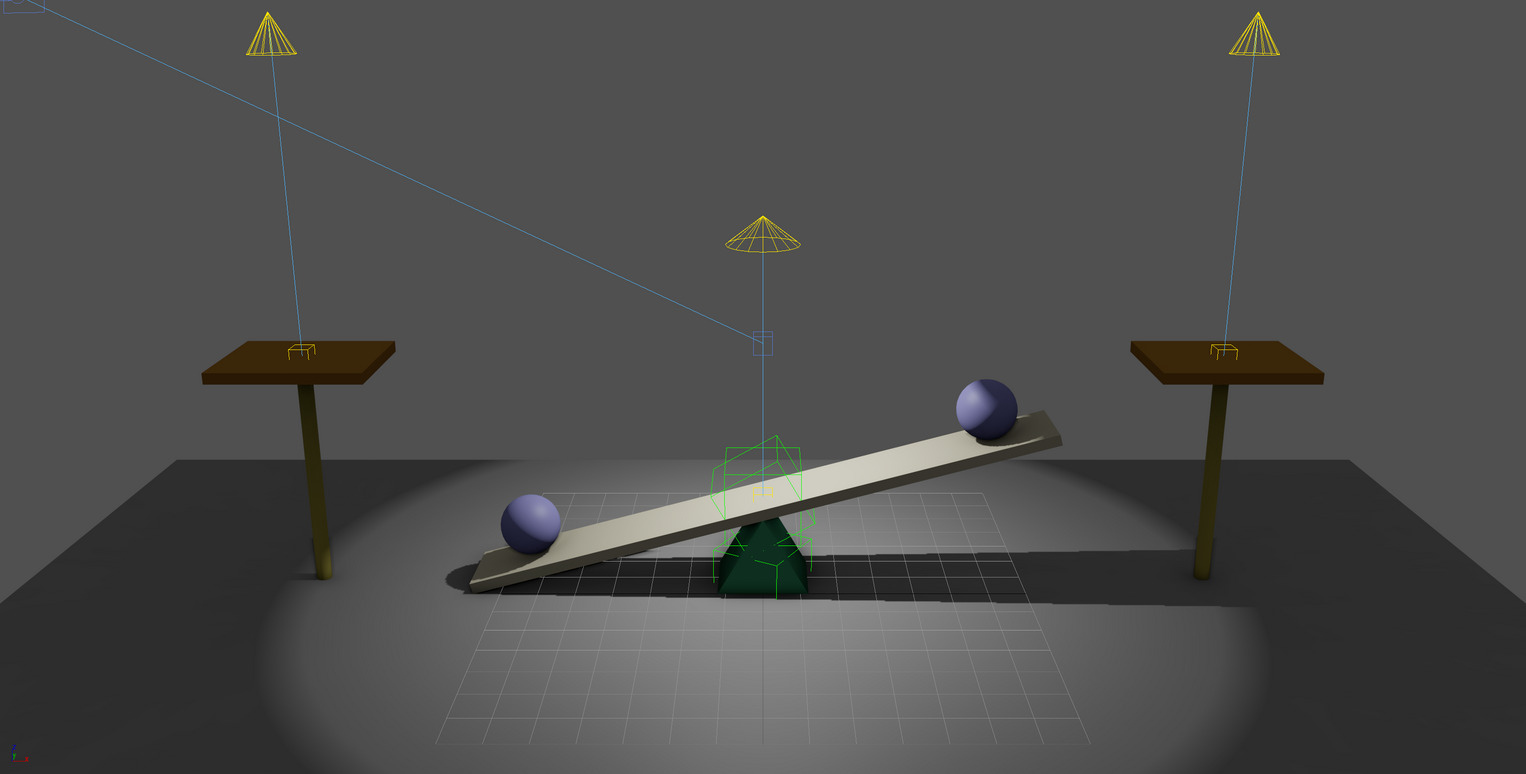
\includegraphics[width=\textwidth]{imagenes/animaciones/general/92.jpg}
    \caption{Animación de la escena en el instante 92.}
 \end{subfigure}
\hfill
 \begin{subfigure}[t]{0.48\textwidth}
    \centering
    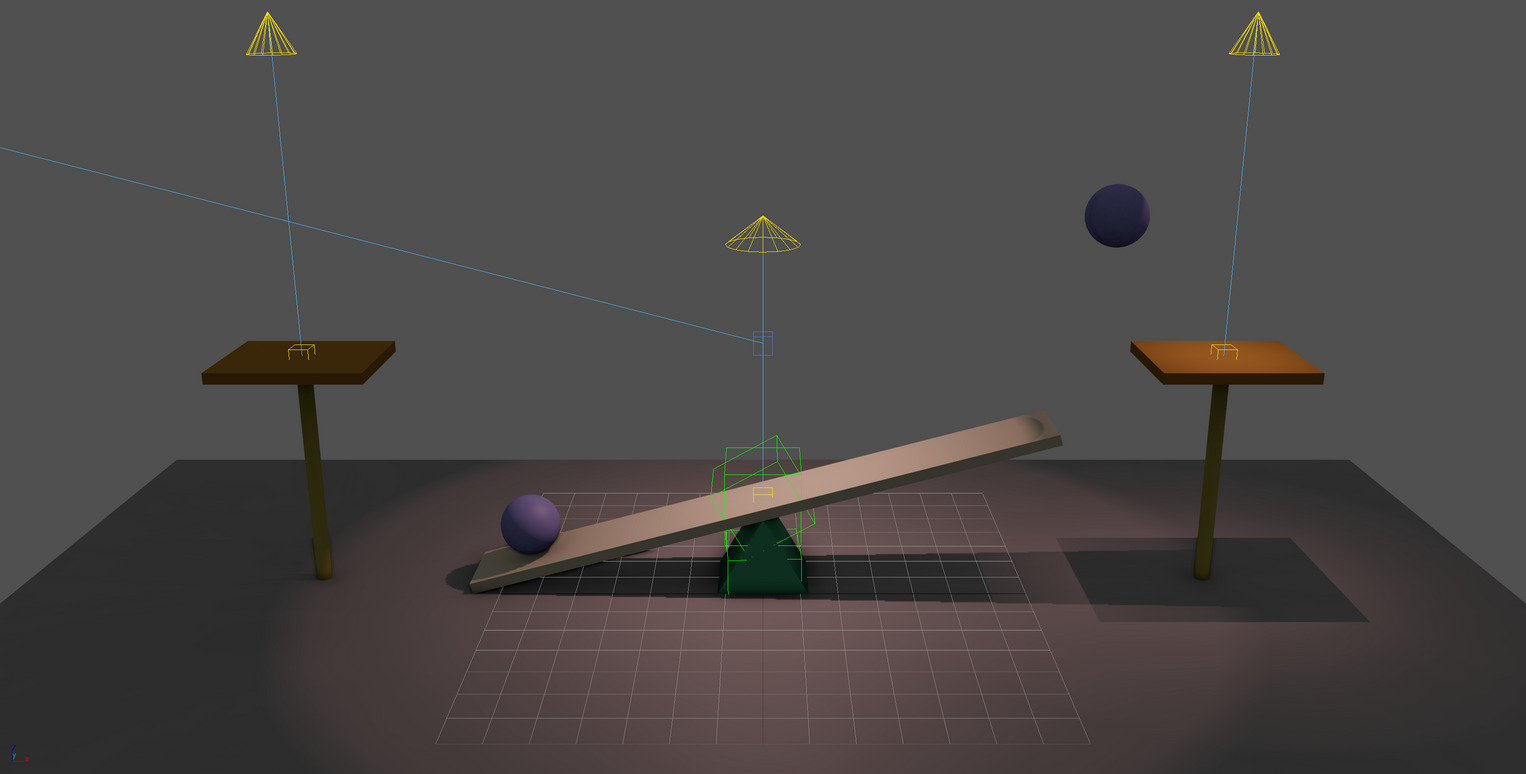
\includegraphics[width=\textwidth]{imagenes/animaciones/general/102.jpg}
    \caption{Animación de la escena en el instante 102.}
 \end{subfigure}
\hfill
 \begin{subfigure}[t]{0.48\textwidth}
    \centering
    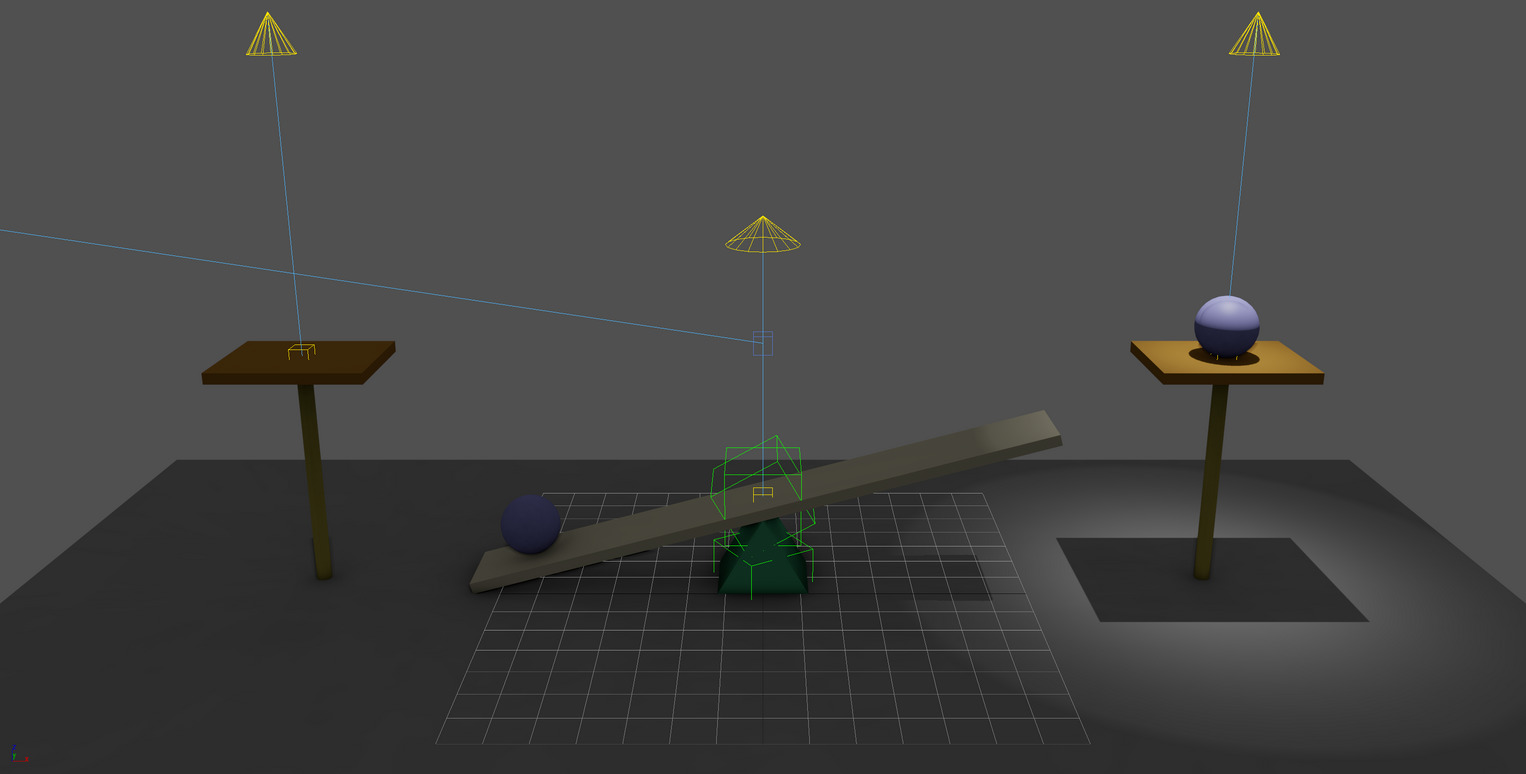
\includegraphics[width=\textwidth]{imagenes/animaciones/general/112.jpg}
    \caption{Animación de la escena en el instante 112.}
 \end{subfigure}
\hfill
 \begin{subfigure}[t]{0.48\textwidth}
    \centering
    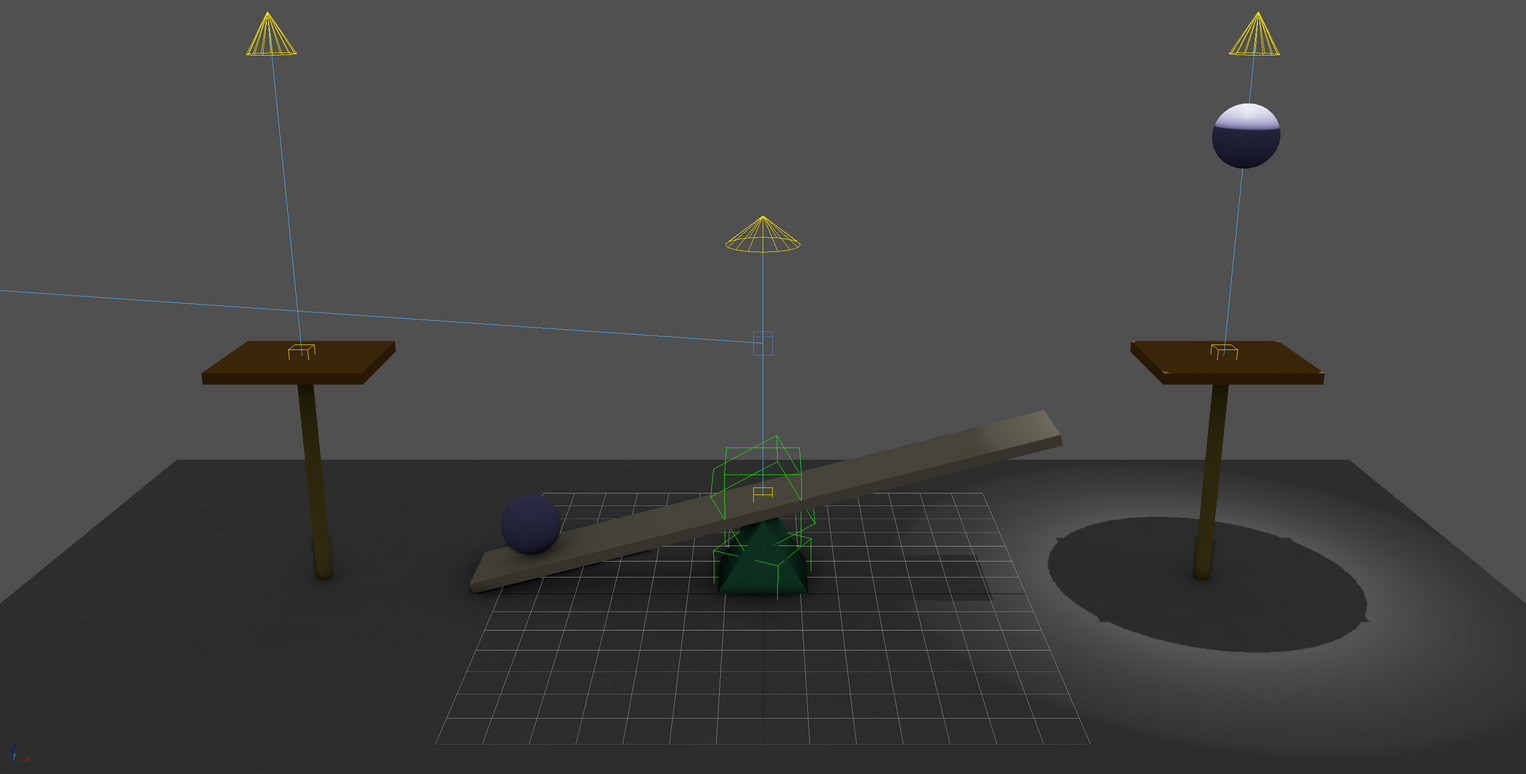
\includegraphics[width=\textwidth]{imagenes/animaciones/general/124.jpg}
    \caption{Animación de la escena en el instante 124.}
 \end{subfigure}
\end{figure}

\begin{figure}[H]\ContinuedFloat
 \begin{subfigure}[t]{0.48\textwidth}
    \centering
    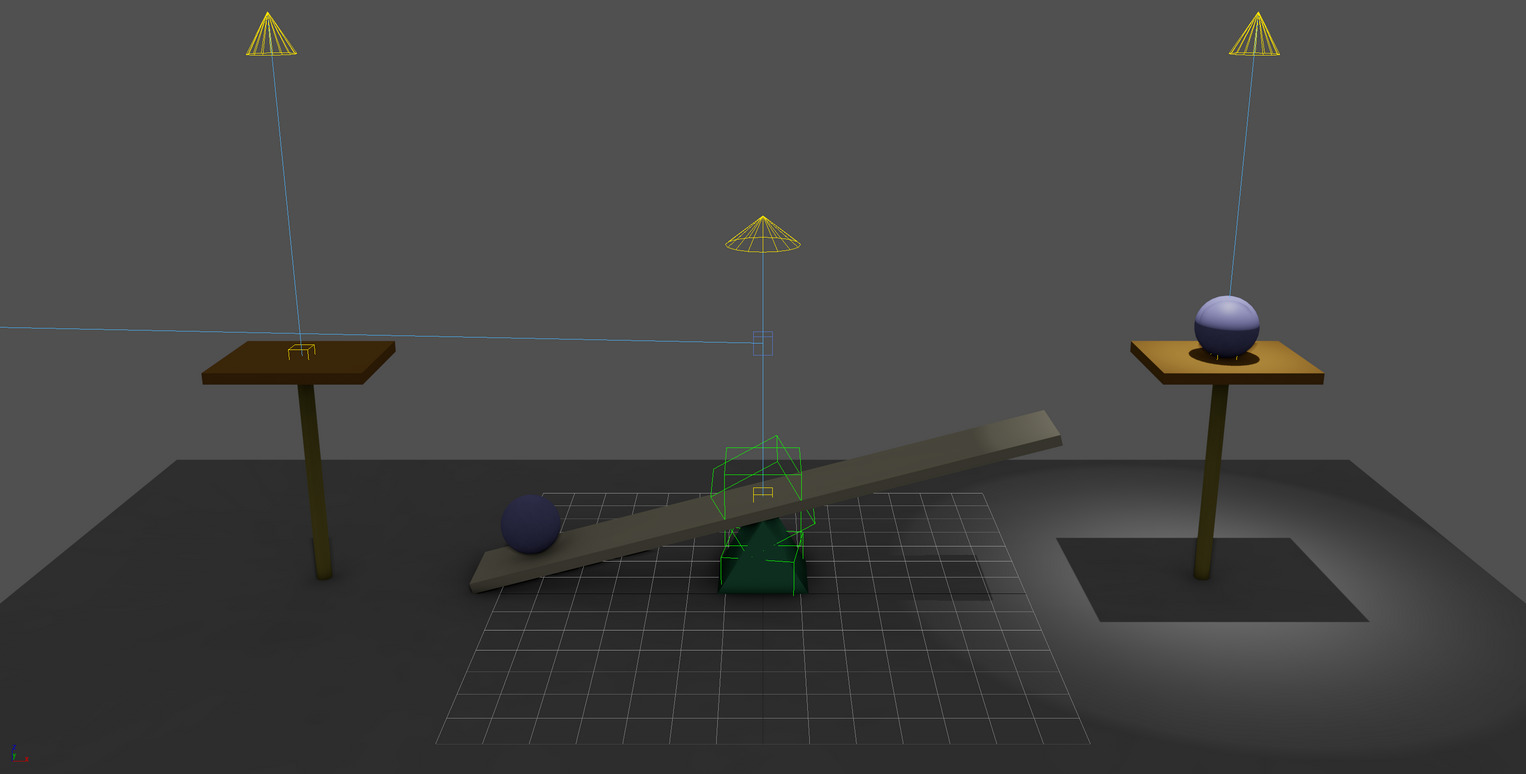
\includegraphics[width=\textwidth]{imagenes/animaciones/general/136.jpg}
    \caption{Animación de la escena en el instante 136.}
 \end{subfigure}
\hfill
 \begin{subfigure}[t]{0.48\textwidth}
    \centering
    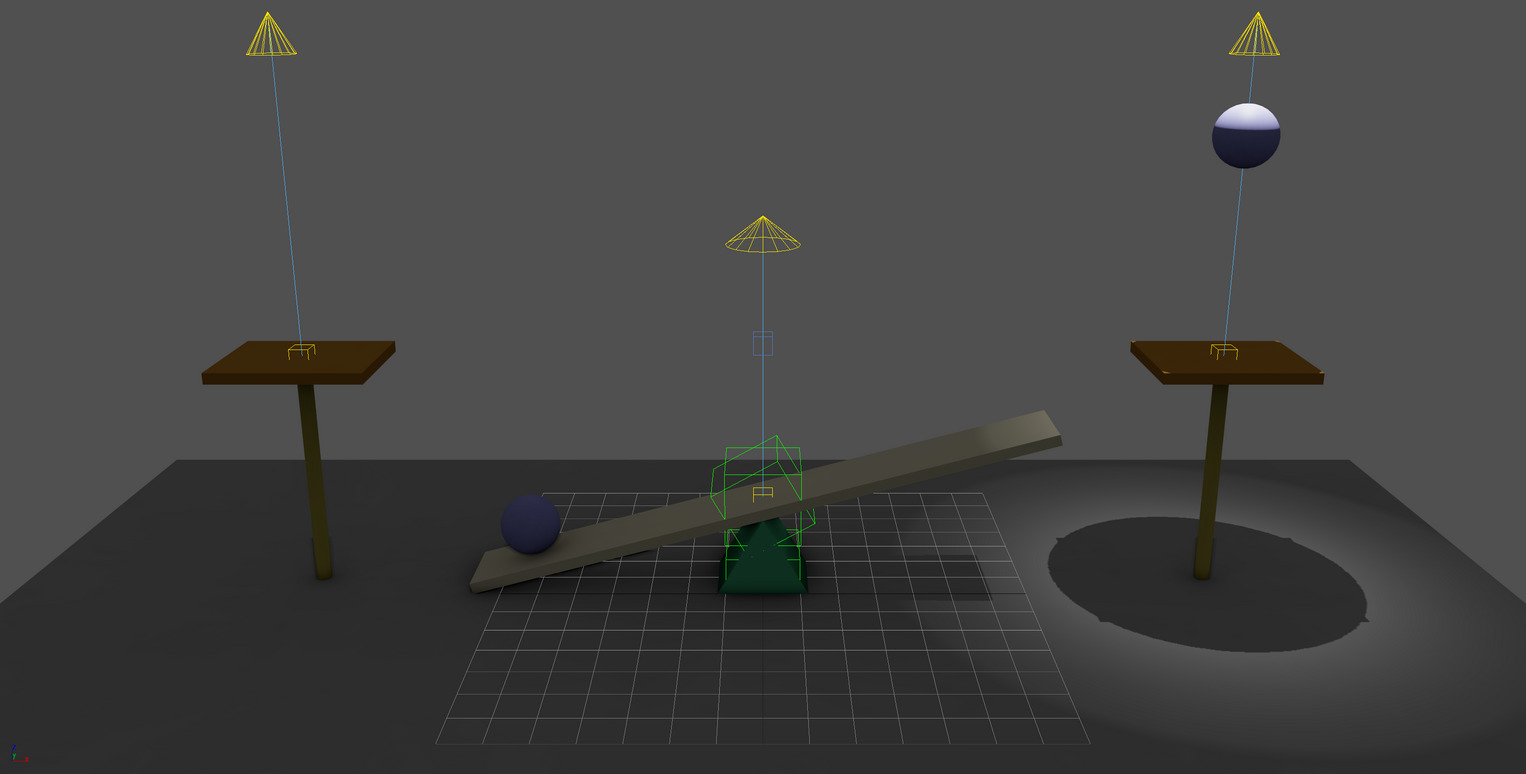
\includegraphics[width=\textwidth]{imagenes/animaciones/general/150.jpg}
    \caption{Animación de la escena en el instante 150.}
 \end{subfigure}
 \caption{Instantes más importantes de la animación resultante.}
\end{figure}